\documentclass[12pt, notitlepage]{article}
\usepackage[margin=1in, top=0.5in]{geometry}
\usepackage[utf8x]{inputenc}
\usepackage{gensymb}
\usepackage{array}
\usepackage{amssymb}
\usepackage{amsmath}
\usepackage{graphicx}
\usepackage{tabularx}
\usepackage{pbox}
\usepackage[makeroom]{cancel}
\usepackage{float}
\usepackage{caption}
\usepackage{newfloat}
\DeclareFloatingEnvironment[name={Gráfico}]{graph}
\newcommand\numberthis{\addtocounter{equation}{1}\tag{\theequation}}

\title{Título}

\date{\today}
\renewcommand\refname{Referencias}
\renewcommand\tablename{Tabla}
\renewcommand\figurename{Figura}
\newcommand{\norm}[1]{\left\lVert#1\right\rVert}

\geometry{letterpaper}

\begin{document}
\thispagestyle{empty}
\setlength{\unitlength}{1 cm} %Especificar unidad de trabajo
\begin{picture}(18,4)
\put(0,0){
\includegraphics[scale=0.38]{UTFSM_logo.png}}
\put(11.5,0){
\includegraphics[scale=0.2]{mecusm.jpg}}
\end{picture}
\\
\\
\begin{center}
{\LARGE {Universidad Técnica Federico Santa María}}\\[0.5cm]
{\Large Departamento de Ingeniería Mecánica}\\[2cm]
%{\Large Redes}\\[2.3cm]
{\Huge \textbf{Tarea 2: }}\\[0.2cm]
{\Huge \textbf{``Resolución de sistemas de ecuaciones lineales."}}\\[0.2cm]
{\large IPM-458 - Computación Científica.}\\
{\large Alumno: Nicolás Espinoza M.}\\[6cm]
Profesor: Franco Perazzo M.\\
Ayudante: Luis Fuenzalida L.\\[3cm]
Valparaíso - Mayo 12, 2017
\end{center}
\newpage
\tableofcontents
\newpage

\section{Introducción al Problema.}

El desarrollo de este informe gira en torno a un gancho de grúa de sección variable. De la forma de la sección del gancho se conocen algunos puntos en coordenadas $X-Y$, que gracias a métodos numéricos también permitirán definir la periferia de la sección transversal.\\\\
En el trabajo se utilizan Splines Cúbicos que permiten interpolar curvas a los puntos obtenidos en las mediciones presentadas en la tabla entregada en el problema.\\\\
\subsection{Spline cúbico natural.}

Sirve para interpolar puntos mediante un polinomio cúbico. En casos con múltiples puntos, los coeficientes del polinomio varían en cada intervalo. De manera genérica en un dominio $[a,b]$ con intervalos $[x_i,x_{i+1}]$, los polinomios son de la forma
\begin{gather}
S_i(x_i) = \alpha_i + \beta_i(x-x_i) + \gamma_i(x-x_i)^2 + \delta_i(x-x_i)^3 \\
S_{i+1}(x_{i+1}) = \alpha_{i+1} + \beta_{i+1}(x-x_{i+1}) + \gamma_{i+1}(x-x_{i+1})^2 + \delta_{i+1}(x-x_{i+1})^3
\end{gather}

Ahora, de la evaluación en los puntos sólo se obtienen cuatro condiciones, por lo que faltan al menos otras 4 para esta ecuación:
\begin{itemize}
\item{Primera derivada continua en los puntos: $S_i'(x_i) = S_i'(x_{i+1})$}
\item{Segunda derivada nula en los extremos del dominio de evaluación: $S_i''(a) = S_{i+1}''(b) = 0$}
\end{itemize}

\subsection{Regla de integración de Simpson.}
El método de Simpson consiste en aproximar una integral mediante un promedio ponderado de la evaluación de la función a integrar en tres puntos del intervalo de integración: el extremo inicial $a$, el extremo final $b$ y el punto medio $m$
\begin{equation}
\int_a^b f(x) dx \approx \frac{b-a}{6}\left(f(a) + 4f(m)+f(b)\right)
\end{equation}

\section{Preguntas.}

\subsection{Pregunta 1.}

Se desarrolla un programa en \texttt{FORTRAN 90} que entrega una aproximación mediante splines del valor de $f(x)$ para un x que ingrese el usuario. Para este el programa determina los coeficientes en los distintos intervalos y, dependiendo de en qué rango se encuentre el valor de $x$ ingresado por el usuario, entrega el Spline correspondiente resuelto. Los valores de los coeficientes están en el archivo \texttt{coeficientes.txt}.

\subsection{Pregunta 2.}
A continuación se presentan los gráficos de lo que entrega Excel cuando se interpolan los puntos mediante curvas, y lo que se puede obtener al graficar el resultado de los Splines resueltos en la Pregunta 1.

\begin{figure}[H]
\centering
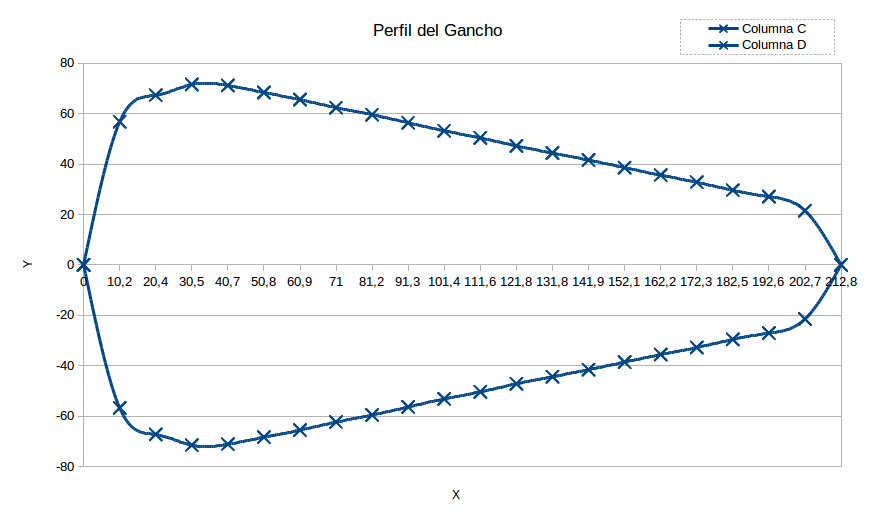
\includegraphics[scale=0.5]{Excel_Gancho.png}
\caption{Resultado de graficar mediante Excel.}
\end{figure}

\begin{figure}[H]
\centering
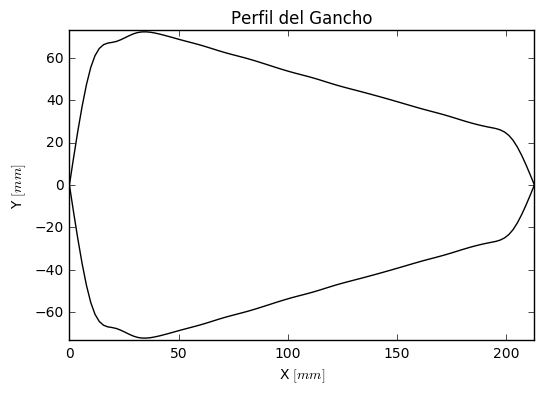
\includegraphics[scale=0.8]{Perfil_Gancho.png}
\caption{Resultado de graficar mediante matplotlib.}
\end{figure}

Se puede apreciar que las figuras coinciden bastante bien, excepto quizás por lo que ocurre entre los puntos 2 y 4, pues se podría argumentar que Excel los suaviza mejor que el Spline. También es importante notar que en el punto más hacia la derecha de la gráfica, la curva no es suave. Esto ocurre porque el Spline se hizo en la mitad superior y luego simplemente se reflejó para obtener la parte inferior.

\subsection{Pregunta 3.}

\section{Conclusiones.}
Las aproximaciones numéricas son de vital importancia en las aplicaciones ingenieriles, pues permiten resolver problemas mediante aproximaciones y, más aún, definir curvas que representan un problema cuando lo único que se tienen son datos. En casos como este último, hasta que se desarrolla una aproximación de curva con la que se pueda trabajar (como el método de Splines, por ejemplo), es poco lo que se puede hacer para trabajar esos datos aislados. Sin embargo, con la interpolación de curvas entre esos datos, se pueden obtener funciones que, en el ejemplo de esta tarea, permiten obtener el perfil de un gancho, su área y sus radios neutro y centroidal.\\\\
Actualmente el uso de los Splines en Ingeniería Mecánica probablemente es más evidente en los sistemas de diseño mecánico asistidos por computadora: Los CAD. Estos software utilizan Splines para trazar superficies, curvas, biseles, etc. Es así que gracias al boom de la tecnología informática, hoy en día se pueden utilizar métodos numéricos de forma masiva en el diseño computacional.

\end{document}